\documentclass[14pt,a4paper]{article}
\usepackage[utf8]{inputenc}
\usepackage[russianb]{babel}
\usepackage[left=1.5cm,right=1.5cm,top=2cm,bottom=2.5cm]{geometry}
\usepackage{setspace}
\usepackage{indentfirst}
\usepackage{amssymb}
\usepackage{amsmath}

\usepackage{array}
\usepackage[pdftex]{graphicx}
\usepackage{comment}
\usepackage[table,xcdraw]{xcolor}


\usepackage{verbatim}


\graphicspath{{images/}}
\renewcommand{\baselinestretch}{1.3}

\begin{document}

В файле приведён фрагмент базы данных «Кондитерские изделия»
о поставках конфет и печенья в магазины районов города. База данных
состоит из трёх таблиц.
Таблица «Движение товаров» содержит записи о поступлении товаров
со склада в магазины в течение августа 2023 г., а также информацию
о проданных товарах. Поле Тип операции содержит значение Поступление
или Продажа, а в соответствующее поле Количество упаковок, шт. внесена
информация о том, сколько упаковок товара поступило в магазин или было
продано по итогам дня. Заголовок таблицы имеет следующий вид.

\begin{center}
    \begin{tabular}{|c|c|c|c|c|c|}
        \hline
        ID операции & Дата & ID магазина & Артикул & Количество упаковок, шт. & Тип операции \\
        \hline
    \end{tabular}
\end{center}

Таблица «Товар» содержит информацию об основных характеристиках
каждого товара. Заголовок таблицы имеет следующий вид.

\begin{center}
    \begin{tabular}{|c|c|c|c|c|c|}
        \hline
        Артикул & Отдел & Наименование товара & Ед\_изм & Количество в упаковке & Цена за упаковку \\
        \hline
    \end{tabular}
\end{center}

Таблица «Магазин» содержит информацию о местонахождении магазинов.
Заголовок таблицы имеет следующий вид.

\begin{center}
    \begin{tabular}{|c|c|c|}
        \hline
        ID магазина & Район & Адрес \\
        \hline
    \end{tabular}
\end{center}

На рисунке приведена схема указанной базы данных.

\begin{center}
    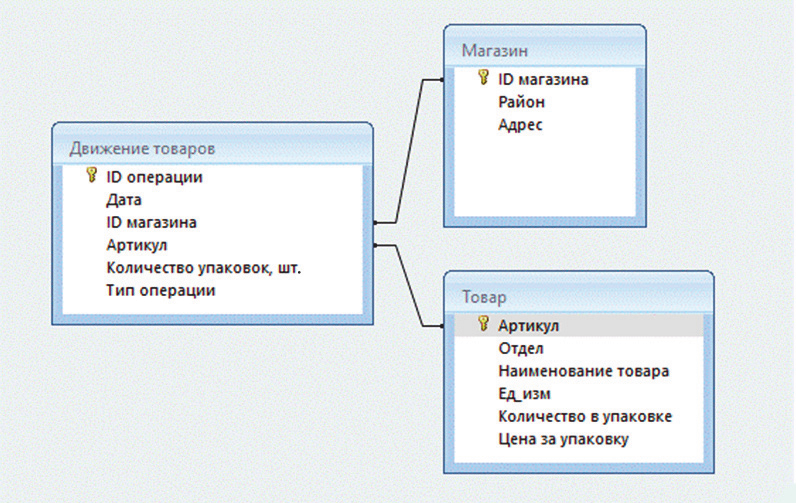
\includegraphics[width=0.6\textwidth]{table.png}
\end{center}

Используя информацию из приведённой базы данных, определите общую
массу (в кг) всех видов зефира, полученных магазинами, расположенными
на проспекте Революции, за период со 2 по 10 августа включительно.
В ответе запишите только число.

\end{document}
